\documentclass[11pt]{article}
\usepackage{fullpage} % changes the margin
\usepackage[pdftex]{graphicx}
\usepackage[
	pdfauthor={Brian Weinstein},
	pdftitle={Homework 1},
	bookmarks=true,
	colorlinks=true,
	linkcolor=blue,
	urlcolor=blue,
	citecolor=blue,
	pdftex,
	linktocpage=true
	]{hyperref}
\usepackage[textsize=tiny]{todonotes}
\usepackage{float}

%\usepackage{fancyhdr}
%\usepackage{amssymb}
%\pagestyle{fancy}
%\lhead{Homework 01}
%\chead{Brian Weinstein}
%\rhead{STAT S4240 002}



\begin{document}

\noindent
\large\textbf{STAT S4240 002, Homework 1} \hfill \textbf{Brian Weinstein}\\
\normalsize 13 July, 2015 \hfill  bmw2148\\


\section*{Problem 1: \href{http://www-bcf.usc.edu/~gareth/ISL/}{James} 2.4, Exercise 8}

\subsection*{Part a}

\begin{figure}[H]
	\centering
	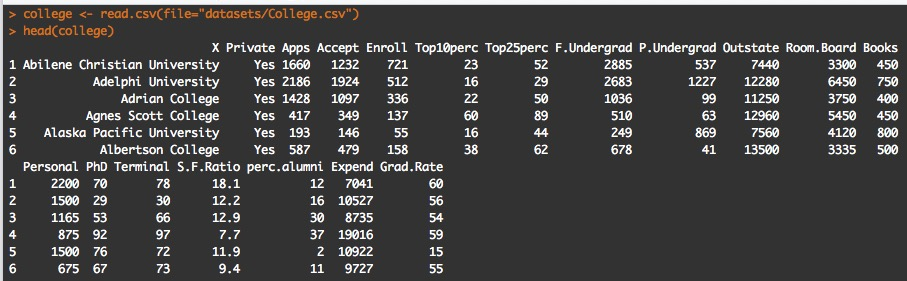
\includegraphics[width=6.5in]{8a.jpeg}
	%\caption{}
	%\label{fig:figName}
\end{figure}


\subsection*{Part b}

\begin{figure}[H]
	\centering
	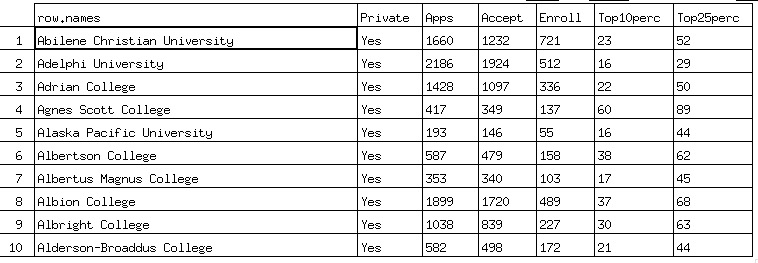
\includegraphics[width=6.5in]{8b.jpeg}
	%\caption{}
	%\label{fig:figName}
\end{figure}

\subsection*{Part c}

\subsubsection*{Part i}

\begin{figure}[H]
	\centering
	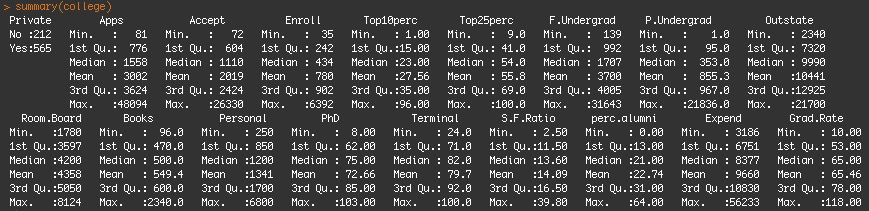
\includegraphics[width=6.5in]{8ci.jpeg}
	%\caption{}
	%\label{fig:figName}
\end{figure}

\subsubsection*{Part ii}

\begin{figure}[H]
	\centering
	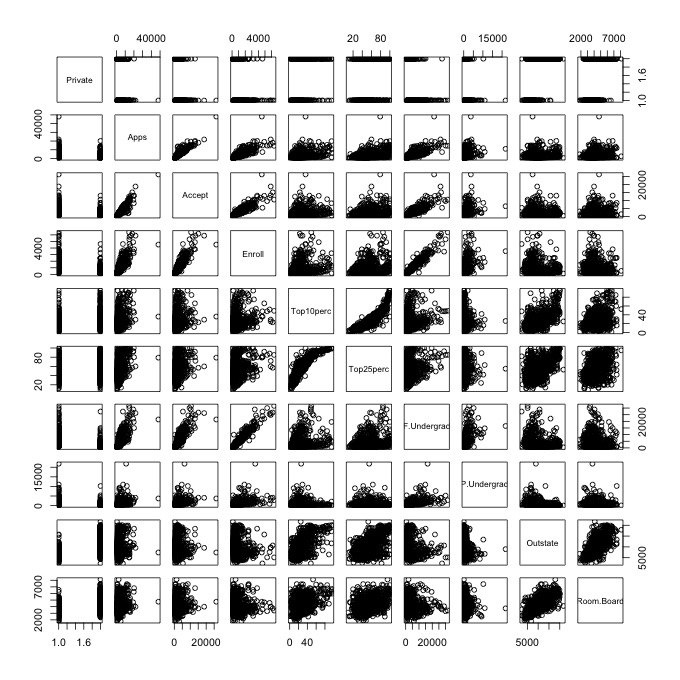
\includegraphics[width=5.5in]{8cii.jpeg}
	%\caption{}
	%\label{fig:figName}
\end{figure}

\subsubsection*{Part iii}

\begin{figure}[H]
	\centering
	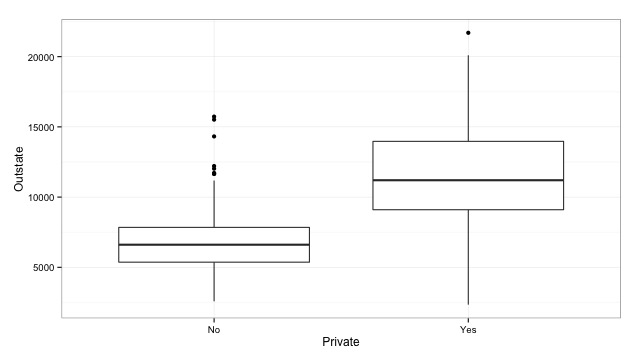
\includegraphics[width=6.5in]{8ciii.jpeg}
	%\caption{}
	%\label{fig:figName}
\end{figure}

\subsubsection*{Part iv}

There are 78 colleges categorized as "Elite".

\begin{figure}[H]
	\centering
	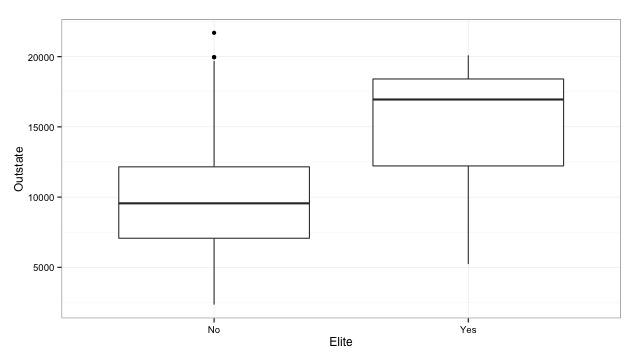
\includegraphics[width=6.5in]{8civ.jpeg}
	%\caption{}
	%\label{fig:figName}
\end{figure}

\subsubsection*{Part v}

\begin{figure}[H]
	\centering
	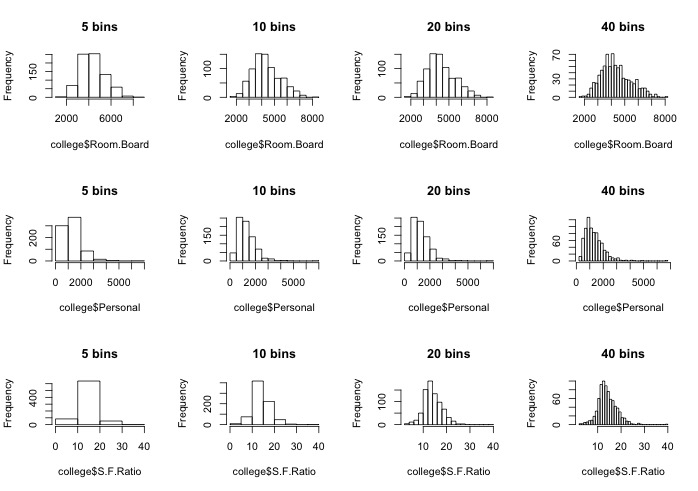
\includegraphics[width=6.5in]{8cv.jpeg}
	%\caption{}
	%\label{fig:figName}
\end{figure}

\subsubsection*{Part vi}

I chose to explore acceptance and enrollment rates, with acceptance rate defined as the number of students accepted per application received (\texttt{college\$Accept/college\$Apps}), and enrollment rate defined as the number of students enrolled per applicant accepted (\texttt{college\$Enroll/college\$Accept}).

\begin{figure}[H]
	\centering
	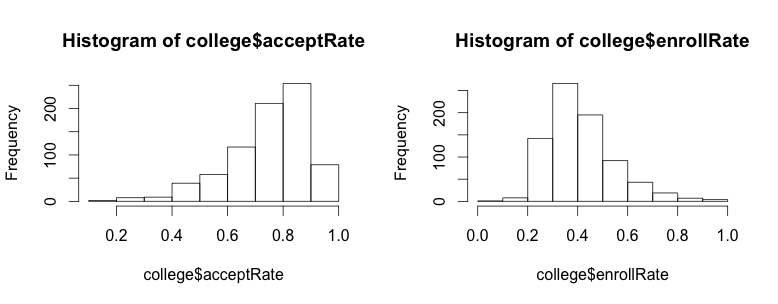
\includegraphics[width=5.5in]{8cvi_histograms.png}
	%\caption{}
	%\label{fig:figName}
\end{figure}

Somewhat surprisingly, there's little correlation between acceptance and enrollment rate.
\begin{verbatim}
> cor(college$acceptRate, college$enrollRate)
[1] 0.0824304
\end{verbatim}

\begin{figure}[H]
	\centering
	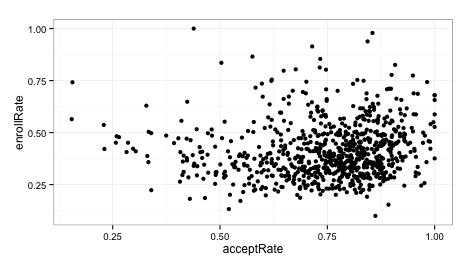
\includegraphics[width=5.5in]{8cvi_enroll_vs_accept.png}
	%\caption{}
	%\label{fig:figName}
\end{figure}


I also looked at summary statistics by public vs private schools.
\begin{verbatim}
> college %>%
+   group_by(Private) %>%
+   summarize(min.acceptRate=min(acceptRate),
+             median.acceptRate=median(acceptRate),
+             mean.acceptRate=mean(acceptRate),
+             max.acceptRate=max(acceptRate),
+             min.enrollRate=min(enrollRate),
+             median.enrollRate=median(enrollRate),
+             mean.enrollRate=mean(enrollRate),
+             max.enrollRate=max(enrollRate)) %>%
+   as.data.frame()


  Private min.acceptRate median.acceptRate mean.acceptRate max.acceptRate min.enrollRate
1      No      0.3397060         0.7443387       0.7265305              1     0.13242009
2     Yes      0.1544863         0.7885653       0.7545812              1     0.09975397
  median.enrollRate mean.enrollRate max.enrollRate
1         0.4405908       0.4620216      0.9382716
2         0.3660934       0.3932510      1.0000000
\end{verbatim}



\begin{figure}[H]
	\centering
	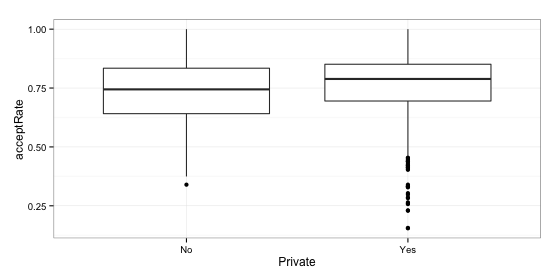
\includegraphics[width=5.5in]{8cvi_acceptRate_boxplots.png}
	%\caption{}
	%\label{fig:figName}
\end{figure}

\begin{figure}[H]
	\centering
	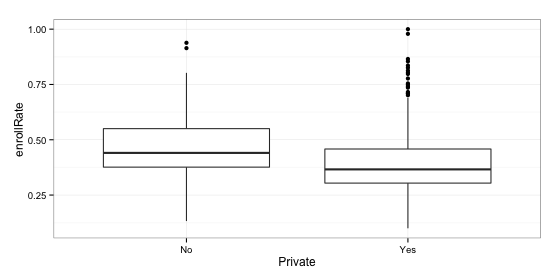
\includegraphics[width=5.5in]{8cvi_enrollRate_boxplots.png}
	%\caption{}
	%\label{fig:figName}
\end{figure}



\section*{Problem 2: \href{http://www-bcf.usc.edu/~gareth/ISL/}{James} 2.4, Exercise 9}



















\end{document}